\section{Introduction}

\begin{figure}[!tbp]
\centering
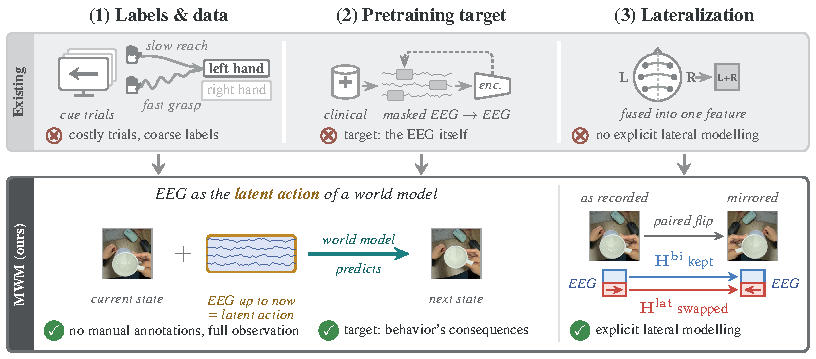
\includegraphics[width=\linewidth]{MWM/figures/mwm_teaser.pdf}
\caption{\textbf{Existing approaches (top) versus \mwm{} (bottom) on the three challenges of motor EEG representation learning.}
\textbf{(1)} Cue-based trials are costly to scale, and categorical labels give one class to movements that unfold differently~\citep{tangermann2012review,schirrmeister2017deep,lawhern2018eegnet}.
\textbf{(2)} General-purpose EEG foundation models (FMs) pretrain with EEG-only objectives~\citep{kostas2021bendr,jiang2024large,wang2025cbramod}.
\mwm{} answers both with one mechanism: it treats the EEG recorded up to the current frame as the latent action of a world model that predicts the next visual state. It therefore learns from naturalistic EEG and egocentric video without action annotations, and its target is the visual consequence of behavior rather than the EEG itself.
\textbf{(3)} Existing methods do not explicitly separate bilateral from lateral activity~\citep{schirrmeister2017deep,lawhern2018eegnet,wang2025cbramod}; \mwm{} does, and pairs each horizontal video mirror with an exchange of only the lateral component $\mathbf{H}^{\mathrm{lat}}$.}
\label{fig:mwm-teaser}
\end{figure}

Motor decoding from electroencephalography (EEG) aims to infer intended or executed movements from non-invasive recordings of brain activity. It encompasses both recognizing movement categories and estimating continuous quantities such as movement trajectories and force. This capability underpins brain--computer interfaces for assistive control and neurorehabilitation, allowing movement-related neural activity to guide external devices or rehabilitation feedback~\citep{tangermann2012review,ramos2013brain}. For these applications, useful EEG representations must capture both which movement is intended and how it unfolds, and transfer across motor tasks with limited labeled data. Learning such representations presents three challenges (Figure~\ref{fig:mwm-teaser}, top).

First, task-specific motor decoding faces limitations in both data scalability and the information conveyed by supervision. Supervised motor-decoding research is largely organized around labeled examples of predefined tasks, commonly collected through repeated, cue-based laboratory trials~\citep{tangermann2012review,schirrmeister2017deep,lawhern2018eegnet}. Such protocols make it costly to expand the volume and diversity of training data. Moreover, categorical annotations such as ``left hand'' and ``right hand'' compress motor behavior into a small vocabulary. Movements with different trajectories, speeds, or forces can share the same label, leaving their within-class variation unspecified by the training target. Direct measurements of continuous kinematics or force retain such within-class variation, but collecting them at scale typically requires task-specific instrumentation and careful synchronization with EEG. Thus, scaling motor representation learning requires both more accessible collection paradigm and supervision that retains information beyond discrete action categories.

Second, general-purpose EEG foundation models address label scarcity through self-supervised objectives such as contrastive learning, masked signal reconstruction, and neural token prediction~\citep{kostas2021bendr,chien2022maeeg,jiang2024large,wang2024eegpt,wang2025cbramod}. Although these objectives learn useful signal structure, they do not directly supervise the relationship between neural activity and movement. Their pretraining corpora are also assembled primarily for broad or clinical EEG analysis rather than for capturing continuous, naturalistic motor behavior and its consequences~\citep{jiang2024large,wang2025cbramod,obeid2016tuh,ouahidi2025reve}. These differences motivate pretraining that aligns both the learning signal and the recording context with motor decoding.

Third, motor EEG exhibits \emph{lateralization}: similar movement-related patterns can indicate different acting sides depending on which hemisphere they occur in. For example, sensorimotor rhythm suppression is often stronger over the left hemisphere for right-hand movements and vice versa~\citep{pfurtscheller1997motor,nam2011lateralization}. Without this structural prior, existing encoders~\citep{schirrmeister2017deep,lawhern2018eegnet,wang2025cbramod} must learn the relationship between patterns and hemispheric location from data, potentially requiring larger training datasets and yielding suboptimal decoding performance when data are limited.

World-model training faces a similar bottleneck in scaling data collection. Instrumented interfaces can constrain natural behavior and capture only selected aspects of action. For example, handheld grippers and motion-capture gloves primarily record hand kinematics, without directly measuring head and leg movements, interaction forces, or hand stiffness~\citep{chi2024umi,wang2024dexcap}. Video-based approaches instead infer pseudo-actions from current and future frames~\citep{bruce2024genie,gao2025adaworld}. However, access to future frames introduces a risk of target-information leakage: pseudo-actions may encode future visual content, allowing the world model to exploit prediction shortcuts rather than learn transferable action-conditioned dynamics~\citep{garrido2026lawm}.

To address these challenges, we propose the Mind World Model (\mwm{}), which jointly learns a mind model and a world model from synchronized EEG and egocentric video in EgoBrain~\citep{lin2026egobrain}. The mind model maps EEG observed up to the current frame to a latent action, and the world model uses it to predict a future visual representation. Using egocentric recordings of natural motor behavior, rather than general-purpose EEG corpora, aligns the training data with motor decoding. Visual prediction supplies supervision beyond categorical labels without task-specific annotation, enabling scalable pretraining. Encoding actions from EEG avoids explicit motion measurements and future-frame leakage. Joint learning thus produces action-related EEG representations and a world-model initialization for future prediction conditioned on real actions.

To capture motor lateralization, we introduce the Lateralization-Aware Transformer (LAT), an EEG encoder that uses frame averaging~\citep{puny2022frame} over original and mirrored representations to separate shared bilateral features from side-specific lateral features. When a video is mirrored horizontally, LAT exchanges lateral EEG features across homologous electrodes while preserving the bilateral component. This prior links corresponding movement patterns across hemispheres, reducing the burden of learning their left--right relationship from limited data.

Our contributions are as follows:
\begin{itemize}
    \item We introduce \mwm{}, which learns motor EEG representations from naturalistic EEG--video by predicting the visual consequences of behavior. This objective provides supervision beyond categorical action labels and enables scalable data collection without explicit action annotations.
    \item We propose LAT to encode hemispheric correspondence by separating bilateral and lateral EEG features, reducing the burden of learning this structure from data.
    \item We show that the pretrained world model transfers from EEG-derived actions to prediction conditioned on real actions, opening a path to scalable world-model data collection without relying on manipulation interfaces that constrain natural behavior and capture only selected aspects of action.
\end{itemize}

We evaluate the mind model on \mwmClsTasks{} classification and \mwmRegTasks{} regression tasks, and the world model on future prediction conditioned on real actions. Relative to the strongest baseline in each task family, the mind model improves task-averaged balanced accuracy by \mwmClsGainPct{}\% and Pearson correlation by \mwmRegGainPct{}\%. Ablations show that alignment, prediction, and frame averaging each improve average transfer, with effects that vary by task. Relative to the latent-action baseline, the world model reduces L1 error by \mwmWMWithinGainPct{}\% within recordings and \mwmWMSubjectGainPct{}\% on held-out subjects.
